\documentclass[14pt]{extbook}
\usepackage{multicol, enumerate, enumitem, hyperref, color, soul, setspace, parskip, fancyhdr} %General Packages
\usepackage{amssymb, amsthm, amsmath, latexsym, units, mathtools} %Math Packages
\everymath{\displaystyle} %All math in Display Style
% Packages with additional options
\usepackage[headsep=0.5cm,headheight=12pt, left=1 in,right= 1 in,top= 1 in,bottom= 1 in]{geometry}
\usepackage[usenames,dvipsnames]{xcolor}
\usepackage{dashrule}  % Package to use the command below to create lines between items
\newcommand{\litem}[1]{\item#1\hspace*{-1cm}\rule{\textwidth}{0.4pt}}
\pagestyle{fancy}
\lhead{Progress Quiz 6}
\chead{}
\rhead{Version ALL}
\lfoot{4563-7456}
\cfoot{}
\rfoot{Summer C 2021}
\begin{document}

\begin{enumerate}
\litem{
First, find the equation of the line containing the two points below. Then, write the equation in the form $ y=mx+b $ and choose the intervals that contain $m$ and $b$.\[ (-4, 2) \text{ and } (-9, -2) \]\begin{enumerate}[label=\Alph*.]
\item \( m \in [0.02, 1.65] \hspace*{3mm} b \in [5.8, 6.08] \)
\item \( m \in [-1.11, 0.12] \hspace*{3mm} b \in [-9.6, -8.37] \)
\item \( m \in [0.02, 1.65] \hspace*{3mm} b \in [6.76, 7.15] \)
\item \( m \in [0.02, 1.65] \hspace*{3mm} b \in [5.11, 5.34] \)
\item \( m \in [0.02, 1.65] \hspace*{3mm} b \in [-5.6, -4.65] \)

\end{enumerate} }
\litem{
Solve the linear equation below. Then, choose the interval that contains the solution.\[ \frac{5x + 9}{6} - \frac{-7x -7}{3} = \frac{7x + 7}{4} \]\begin{enumerate}[label=\Alph*.]
\item \( x \in [1.67, 1.93] \)
\item \( x \in [-1.71, -0.62] \)
\item \( x \in [-0.54, -0.26] \)
\item \( x \in [-6.82, -5.13] \)
\item \( \text{There are no real solutions.} \)

\end{enumerate} }
\litem{
Write the equation of the line in the graph below in Standard Form $Ax+By=C$. Then, choose the intervals that contain $A, B, \text{ and } C$.
\begin{center}
    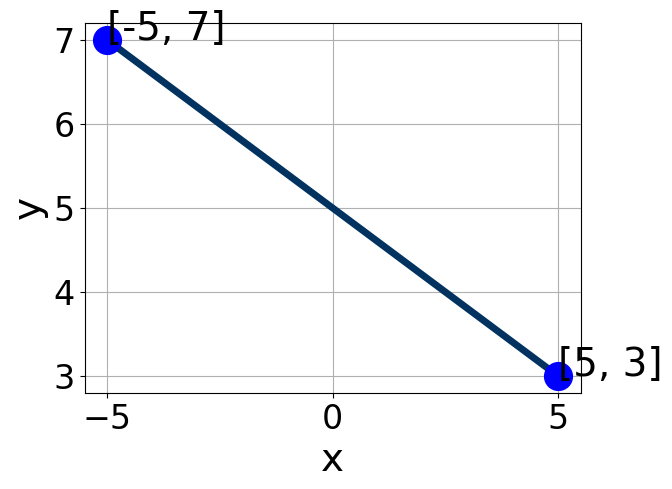
\includegraphics[width=0.5\textwidth]{../Figures/linearGraphToStandardA.png}
\end{center}
\begin{enumerate}[label=\Alph*.]
\item \( A \in [-0.6, 1.4], \hspace{3mm} B \in [-0.15, 2.2], \text{ and } \hspace{3mm} C \in [4, 9] \)
\item \( A \in [2, 9], \hspace{3mm} B \in [4.62, 5.45], \text{ and } \hspace{3mm} C \in [23, 27] \)
\item \( A \in [-0.6, 1.4], \hspace{3mm} B \in [-1.03, 0.21], \text{ and } \hspace{3mm} C \in [-5, -4] \)
\item \( A \in [2, 9], \hspace{3mm} B \in [-7.61, -3.85], \text{ and } \hspace{3mm} C \in [-30, -21] \)
\item \( A \in [-2, -1], \hspace{3mm} B \in [-7.61, -3.85], \text{ and } \hspace{3mm} C \in [-30, -21] \)

\end{enumerate} }
\litem{
Solve the equation below. Then, choose the interval that contains the solution.\[ -13(-4x -5) = -18(-19x -12) \]\begin{enumerate}[label=\Alph*.]
\item \( x \in [0.85, 1.05] \)
\item \( x \in [-0.63, -0.31] \)
\item \( x \in [-1.19, -0.82] \)
\item \( x \in [-0.8, -0.66] \)
\item \( \text{There are no real solutions.} \)

\end{enumerate} }
\litem{
Find the equation of the line described below. Write the linear equation in the form $ y=mx+b $ and choose the intervals that contain $m$ and $b$.\[ \text{Parallel to } 3 x - 8 y = 15 \text{ and passing through the point } (-3, -9). \]\begin{enumerate}[label=\Alph*.]
\item \( m \in [-0.75, 0.37] \hspace*{3mm} b \in [-10.3, -9.3] \)
\item \( m \in [0.31, 1.13] \hspace*{3mm} b \in [6.6, 10] \)
\item \( m \in [0.31, 1.13] \hspace*{3mm} b \in [-8.7, -7.1] \)
\item \( m \in [0.31, 1.13] \hspace*{3mm} b \in [-6.7, -5.4] \)
\item \( m \in [1.83, 2.85] \hspace*{3mm} b \in [-8.7, -7.1] \)

\end{enumerate} }
\litem{
Write the equation of the line in the graph below in Standard Form $Ax+By=C$. Then, choose the intervals that contain $A, B, \text{ and } C$.
\begin{center}
    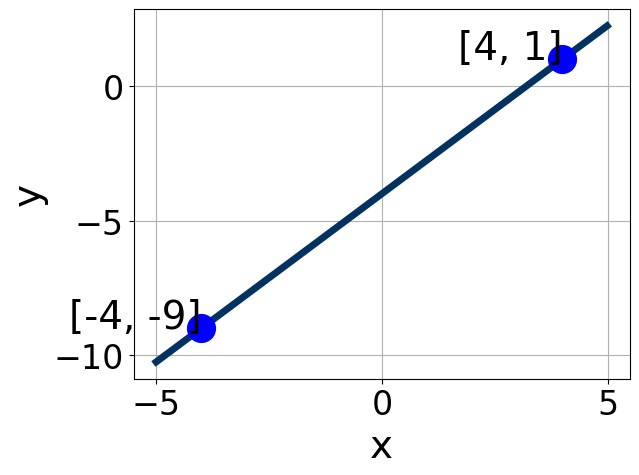
\includegraphics[width=0.5\textwidth]{../Figures/linearGraphToStandardCopyA.png}
\end{center}
\begin{enumerate}[label=\Alph*.]
\item \( A \in [2, 9], \hspace{3mm} B \in [2.7, 6.6], \text{ and } \hspace{3mm} C \in [-17, -15] \)
\item \( A \in [-8, -4], \hspace{3mm} B \in [2.7, 6.6], \text{ and } \hspace{3mm} C \in [-17, -15] \)
\item \( A \in [-4.25, 3.75], \hspace{3mm} B \in [-2.8, 0.8], \text{ and } \hspace{3mm} C \in [1, 6] \)
\item \( A \in [-4.25, 3.75], \hspace{3mm} B \in [0.1, 2.1], \text{ and } \hspace{3mm} C \in [-11, -3] \)
\item \( A \in [2, 9], \hspace{3mm} B \in [-4.2, -3.2], \text{ and } \hspace{3mm} C \in [14, 20] \)

\end{enumerate} }
\litem{
Find the equation of the line described below. Write the linear equation in the form $ y=mx+b $ and choose the intervals that contain $m$ and $b$.\[ \text{Parallel to } 4 x + 9 y = 13 \text{ and passing through the point } (5, -4). \]\begin{enumerate}[label=\Alph*.]
\item \( m \in [-0.18, 0.74] \hspace*{3mm} b \in [-6.8, -5.7] \)
\item \( m \in [-0.5, 0.02] \hspace*{3mm} b \in [-1, 4.2] \)
\item \( m \in [-0.5, 0.02] \hspace*{3mm} b \in [-12.1, -8.4] \)
\item \( m \in [-3.15, -1.79] \hspace*{3mm} b \in [-2.1, -0.3] \)
\item \( m \in [-0.5, 0.02] \hspace*{3mm} b \in [-2.1, -0.3] \)

\end{enumerate} }
\litem{
Solve the equation below. Then, choose the interval that contains the solution.\[ -2(-18x -9) = -19(-16x -8) \]\begin{enumerate}[label=\Alph*.]
\item \( x \in [-0.57, -0.33] \)
\item \( x \in [0.51, 0.65] \)
\item \( x \in [-0.97, -0.59] \)
\item \( x \in [-0.57, -0.33] \)
\item \( \text{There are no real solutions.} \)

\end{enumerate} }
\litem{
First, find the equation of the line containing the two points below. Then, write the equation in the form $ y=mx+b $ and choose the intervals that contain $m$ and $b$.\[ (-5, -9) \text{ and } (9, -2) \]\begin{enumerate}[label=\Alph*.]
\item \( m \in [0.2, 3] \hspace*{3mm} b \in [-7, -4.5] \)
\item \( m \in [-3.7, 0.4] \hspace*{3mm} b \in [-1, 3] \)
\item \( m \in [0.2, 3] \hspace*{3mm} b \in [6.1, 6.7] \)
\item \( m \in [0.2, 3] \hspace*{3mm} b \in [-12.8, -9.6] \)
\item \( m \in [0.2, 3] \hspace*{3mm} b \in [-4.6, -3.9] \)

\end{enumerate} }
\litem{
Solve the linear equation below. Then, choose the interval that contains the solution.\[ \frac{-5x -4}{2} - \frac{3x -8}{8} = \frac{-9x + 8}{4} \]\begin{enumerate}[label=\Alph*.]
\item \( x \in [-6.3, -4.5] \)
\item \( x \in [0.6, 3.2] \)
\item \( x \in [-9.5, -7.8] \)
\item \( x \in [-7.1, -6.1] \)
\item \( \text{There are no real solutions.} \)

\end{enumerate} }
\litem{
First, find the equation of the line containing the two points below. Then, write the equation in the form $ y=mx+b $ and choose the intervals that contain $m$ and $b$.\[ (6, 6) \text{ and } (9, 11) \]\begin{enumerate}[label=\Alph*.]
\item \( m \in [-7.67, 0.33] \hspace*{3mm} b \in [25.8, 29.2] \)
\item \( m \in [-0.33, 8.67] \hspace*{3mm} b \in [3.7, 5.9] \)
\item \( m \in [-0.33, 8.67] \hspace*{3mm} b \in [-1, 1.2] \)
\item \( m \in [-0.33, 8.67] \hspace*{3mm} b \in [-5.2, -2.9] \)
\item \( m \in [-0.33, 8.67] \hspace*{3mm} b \in [1.1, 2.9] \)

\end{enumerate} }
\litem{
Solve the linear equation below. Then, choose the interval that contains the solution.\[ \frac{3x -5}{4} - \frac{4x -7}{3} = \frac{-8x -9}{8} \]\begin{enumerate}[label=\Alph*.]
\item \( x \in [3.9, 8.9] \)
\item \( x \in [-0.32, 4.68] \)
\item \( x \in [-29.4, -25.4] \)
\item \( x \in [-8.3, -1.3] \)
\item \( \text{There are no real solutions.} \)

\end{enumerate} }
\litem{
Write the equation of the line in the graph below in Standard Form $Ax+By=C$. Then, choose the intervals that contain $A, B, \text{ and } C$.
\begin{center}
    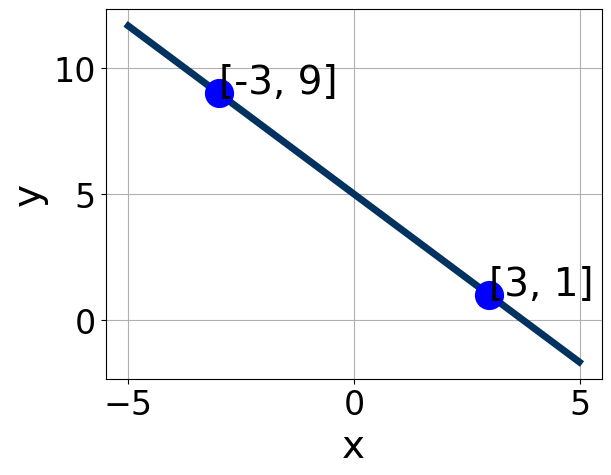
\includegraphics[width=0.5\textwidth]{../Figures/linearGraphToStandardB.png}
\end{center}
\begin{enumerate}[label=\Alph*.]
\item \( A \in [1.6, 5.3], \hspace{3mm} B \in [-3.06, -2.19], \text{ and } \hspace{3mm} C \in [-20, -12] \)
\item \( A \in [1.6, 5.3], \hspace{3mm} B \in [2.68, 3.08], \text{ and } \hspace{3mm} C \in [15, 18] \)
\item \( A \in [1.1, 3.6], \hspace{3mm} B \in [-1.07, -0.62], \text{ and } \hspace{3mm} C \in [-7, 0] \)
\item \( A \in [-9, -3], \hspace{3mm} B \in [-3.06, -2.19], \text{ and } \hspace{3mm} C \in [-20, -12] \)
\item \( A \in [1.1, 3.6], \hspace{3mm} B \in [0.83, 1.71], \text{ and } \hspace{3mm} C \in [1, 13] \)

\end{enumerate} }
\litem{
Solve the equation below. Then, choose the interval that contains the solution.\[ -9(-14x + 11) = -18(7x -6) \]\begin{enumerate}[label=\Alph*.]
\item \( x \in [0.03, 0.04] \)
\item \( x \in [-0.03, 0.01] \)
\item \( x \in [0.82, 0.83] \)
\item \( x \in [-0.07, -0.03] \)
\item \( \text{There are no real solutions.} \)

\end{enumerate} }
\litem{
Find the equation of the line described below. Write the linear equation in the form $ y=mx+b $ and choose the intervals that contain $m$ and $b$.\[ \text{Perpendicular to } 7 x - 4 y = 15 \text{ and passing through the point } (2, -5). \]\begin{enumerate}[label=\Alph*.]
\item \( m \in [0.08, 1.18] \hspace*{3mm} b \in [-6.79, -5.47] \)
\item \( m \in [-1.15, 0.33] \hspace*{3mm} b \in [-7.55, -6.33] \)
\item \( m \in [-1.15, 0.33] \hspace*{3mm} b \in [-4.77, -3.59] \)
\item \( m \in [-1.78, -1] \hspace*{3mm} b \in [-4.77, -3.59] \)
\item \( m \in [-1.15, 0.33] \hspace*{3mm} b \in [3.2, 4.62] \)

\end{enumerate} }
\litem{
Write the equation of the line in the graph below in Standard Form $Ax+By=C$. Then, choose the intervals that contain $A, B, \text{ and } C$.
\begin{center}
    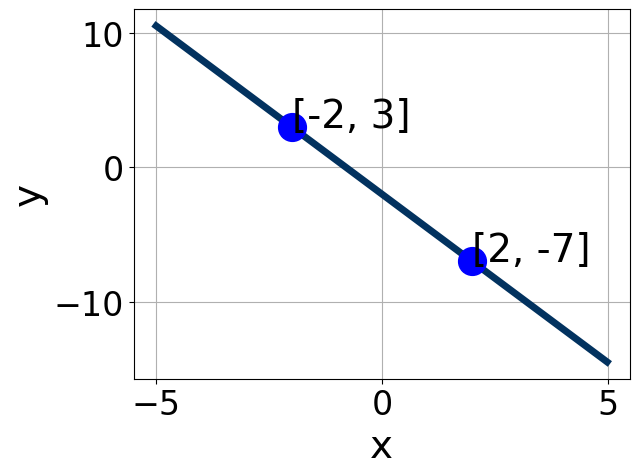
\includegraphics[width=0.5\textwidth]{../Figures/linearGraphToStandardCopyB.png}
\end{center}
\begin{enumerate}[label=\Alph*.]
\item \( A \in [0.4, 4.1], \hspace{3mm} B \in [0.95, 1.55], \text{ and } \hspace{3mm} C \in [-2.54, -1.9] \)
\item \( A \in [-7.1, -3.9], \hspace{3mm} B \in [-2.17, -1.4], \text{ and } \hspace{3mm} C \in [3.28, 4.82] \)
\item \( A \in [4.8, 7.2], \hspace{3mm} B \in [1.19, 2.03], \text{ and } \hspace{3mm} C \in [-5.16, -3.1] \)
\item \( A \in [4.8, 7.2], \hspace{3mm} B \in [-2.17, -1.4], \text{ and } \hspace{3mm} C \in [3.28, 4.82] \)
\item \( A \in [0.4, 4.1], \hspace{3mm} B \in [-1.28, -0.62], \text{ and } \hspace{3mm} C \in [0.68, 2.36] \)

\end{enumerate} }
\litem{
Find the equation of the line described below. Write the linear equation in the form $ y=mx+b $ and choose the intervals that contain $m$ and $b$.\[ \text{Perpendicular to } 5 x + 4 y = 13 \text{ and passing through the point } (4, 7). \]\begin{enumerate}[label=\Alph*.]
\item \( m \in [0.68, 1.24] \hspace*{3mm} b \in [-3.86, -3.23] \)
\item \( m \in [0.68, 1.24] \hspace*{3mm} b \in [3.48, 4.1] \)
\item \( m \in [-1.73, -0.68] \hspace*{3mm} b \in [10.01, 10.27] \)
\item \( m \in [0.82, 1.33] \hspace*{3mm} b \in [3.48, 4.1] \)
\item \( m \in [0.68, 1.24] \hspace*{3mm} b \in [2.56, 3.07] \)

\end{enumerate} }
\litem{
Solve the equation below. Then, choose the interval that contains the solution.\[ -14(-5x -19) = -18(-13x -11) \]\begin{enumerate}[label=\Alph*.]
\item \( x \in [0.1, 0.7] \)
\item \( x \in [-2.5, -0.8] \)
\item \( x \in [1.9, 3] \)
\item \( x \in [-3.4, -2] \)
\item \( \text{There are no real solutions.} \)

\end{enumerate} }
\litem{
First, find the equation of the line containing the two points below. Then, write the equation in the form $ y=mx+b $ and choose the intervals that contain $m$ and $b$.\[ (-2, 11) \text{ and } (-7, -2) \]\begin{enumerate}[label=\Alph*.]
\item \( m \in [1.6, 11.6] \hspace*{3mm} b \in [12.6, 15.6] \)
\item \( m \in [-4.6, 0.4] \hspace*{3mm} b \in [-23.9, -16.6] \)
\item \( m \in [1.6, 11.6] \hspace*{3mm} b \in [-16.3, -16.1] \)
\item \( m \in [1.6, 11.6] \hspace*{3mm} b \in [15, 18.1] \)
\item \( m \in [1.6, 11.6] \hspace*{3mm} b \in [3.5, 6] \)

\end{enumerate} }
\litem{
Solve the linear equation below. Then, choose the interval that contains the solution.\[ \frac{3x -4}{8} - \frac{-8x + 5}{3} = \frac{8x + 7}{5} \]\begin{enumerate}[label=\Alph*.]
\item \( x \in [1.8, 5.3] \)
\item \( x \in [-1.2, 0.6] \)
\item \( x \in [0.6, 2] \)
\item \( x \in [9.2, 12.7] \)
\item \( \text{There are no real solutions.} \)

\end{enumerate} }
\litem{
First, find the equation of the line containing the two points below. Then, write the equation in the form $ y=mx+b $ and choose the intervals that contain $m$ and $b$.\[ (-4, -5) \text{ and } (-8, 4) \]\begin{enumerate}[label=\Alph*.]
\item \( m \in [-5.25, 0.75] \hspace*{3mm} b \in [12.7, 14.1] \)
\item \( m \in [2.25, 6.25] \hspace*{3mm} b \in [19.8, 22.7] \)
\item \( m \in [-5.25, 0.75] \hspace*{3mm} b \in [-2.2, 2] \)
\item \( m \in [-5.25, 0.75] \hspace*{3mm} b \in [-17.3, -13.9] \)
\item \( m \in [-5.25, 0.75] \hspace*{3mm} b \in [11.7, 12.2] \)

\end{enumerate} }
\litem{
Solve the linear equation below. Then, choose the interval that contains the solution.\[ \frac{5x -3}{3} - \frac{9x + 5}{2} = \frac{-3x + 9}{5} \]\begin{enumerate}[label=\Alph*.]
\item \( x \in [-0.3, 0.3] \)
\item \( x \in [-4.5, -0.7] \)
\item \( x \in [-6.6, -4.2] \)
\item \( x \in [-9.5, -7] \)
\item \( \text{There are no real solutions.} \)

\end{enumerate} }
\litem{
Write the equation of the line in the graph below in Standard Form $Ax+By=C$. Then, choose the intervals that contain $A, B, \text{ and } C$.
\begin{center}
    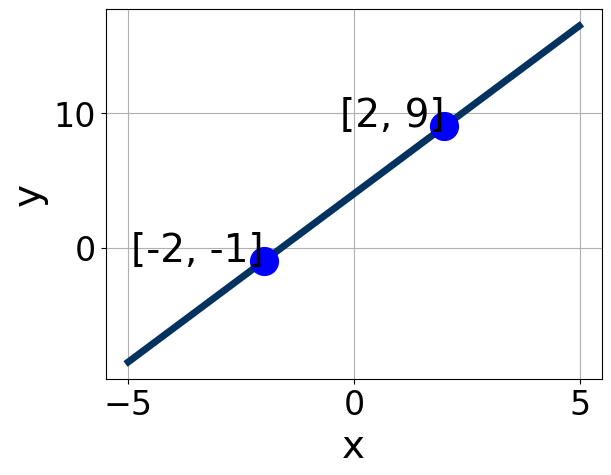
\includegraphics[width=0.5\textwidth]{../Figures/linearGraphToStandardC.png}
\end{center}
\begin{enumerate}[label=\Alph*.]
\item \( A \in [-2.5, 3.5], \hspace{3mm} B \in [-0.1, 1.48], \text{ and } \hspace{3mm} C \in [3, 7] \)
\item \( A \in [-2.5, 3.5], \hspace{3mm} B \in [-1.5, -0.51], \text{ and } \hspace{3mm} C \in [-5, -3] \)
\item \( A \in [4, 6], \hspace{3mm} B \in [1.69, 3.53], \text{ and } \hspace{3mm} C \in [8, 15] \)
\item \( A \in [4, 6], \hspace{3mm} B \in [-2.2, -1.73], \text{ and } \hspace{3mm} C \in [-10, -7] \)
\item \( A \in [-9, -3], \hspace{3mm} B \in [1.69, 3.53], \text{ and } \hspace{3mm} C \in [8, 15] \)

\end{enumerate} }
\litem{
Solve the equation below. Then, choose the interval that contains the solution.\[ -13(5x + 19) = -3(-11x + 15) \]\begin{enumerate}[label=\Alph*.]
\item \( x \in [1.3, 3.6] \)
\item \( x \in [-9.8, -7.4] \)
\item \( x \in [-2.7, -1.6] \)
\item \( x \in [-3.3, -2.5] \)
\item \( \text{There are no real solutions.} \)

\end{enumerate} }
\litem{
Find the equation of the line described below. Write the linear equation in the form $ y=mx+b $ and choose the intervals that contain $m$ and $b$.\[ \text{Parallel to } 5 x - 7 y = 14 \text{ and passing through the point } (10, 3). \]\begin{enumerate}[label=\Alph*.]
\item \( m \in [-1.26, -0.2] \hspace*{3mm} b \in [8.8, 10.4] \)
\item \( m \in [0.07, 1.38] \hspace*{3mm} b \in [-8.4, -4.5] \)
\item \( m \in [0.07, 1.38] \hspace*{3mm} b \in [3.2, 6.7] \)
\item \( m \in [1.02, 1.91] \hspace*{3mm} b \in [-4.3, -1.4] \)
\item \( m \in [0.07, 1.38] \hspace*{3mm} b \in [-4.3, -1.4] \)

\end{enumerate} }
\litem{
Write the equation of the line in the graph below in Standard Form $Ax+By=C$. Then, choose the intervals that contain $A, B, \text{ and } C$.
\begin{center}
    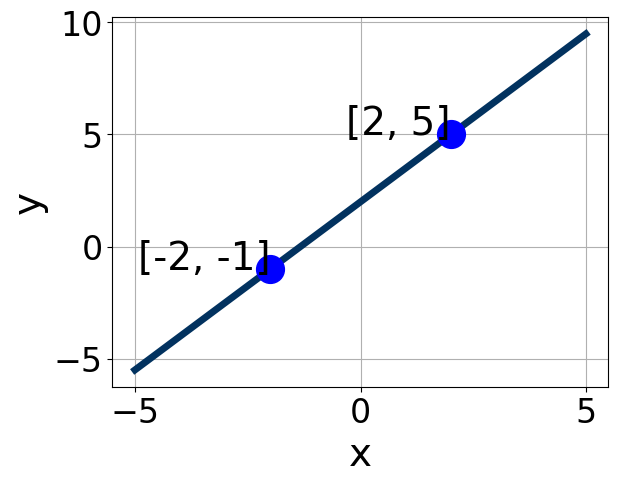
\includegraphics[width=0.5\textwidth]{../Figures/linearGraphToStandardCopyC.png}
\end{center}
\begin{enumerate}[label=\Alph*.]
\item \( A \in [-4.5, -2.5], \hspace{3mm} B \in [1.58, 2.76], \text{ and } \hspace{3mm} C \in [3.79, 5.34] \)
\item \( A \in [-2.8, 0.7], \hspace{3mm} B \in [0.02, 1.16], \text{ and } \hspace{3mm} C \in [0.61, 2.29] \)
\item \( A \in [1, 5.7], \hspace{3mm} B \in [-3.02, -1.46], \text{ and } \hspace{3mm} C \in [-6.48, -3.39] \)
\item \( A \in [-2.8, 0.7], \hspace{3mm} B \in [-1.76, -0.98], \text{ and } \hspace{3mm} C \in [-3.88, -1.87] \)
\item \( A \in [1, 5.7], \hspace{3mm} B \in [1.58, 2.76], \text{ and } \hspace{3mm} C \in [3.79, 5.34] \)

\end{enumerate} }
\litem{
Find the equation of the line described below. Write the linear equation in the form $ y=mx+b $ and choose the intervals that contain $m$ and $b$.\[ \text{Parallel to } 5 x - 7 y = 10 \text{ and passing through the point } (3, 2). \]\begin{enumerate}[label=\Alph*.]
\item \( m \in [1.06, 2.08] \hspace*{3mm} b \in [-0.6, 0.04] \)
\item \( m \in [0.14, 0.72] \hspace*{3mm} b \in [-0.6, 0.04] \)
\item \( m \in [-0.75, -0.33] \hspace*{3mm} b \in [4.03, 4.42] \)
\item \( m \in [0.14, 0.72] \hspace*{3mm} b \in [-1, -0.92] \)
\item \( m \in [0.14, 0.72] \hspace*{3mm} b \in [-0.13, 0.34] \)

\end{enumerate} }
\litem{
Solve the equation below. Then, choose the interval that contains the solution.\[ -6(18x -14) = -10(5x + 7) \]\begin{enumerate}[label=\Alph*.]
\item \( x \in [2.61, 2.82] \)
\item \( x \in [0.18, 0.34] \)
\item \( x \in [-0.04, 0.22] \)
\item \( x \in [-0.6, -0.1] \)
\item \( \text{There are no real solutions.} \)

\end{enumerate} }
\litem{
First, find the equation of the line containing the two points below. Then, write the equation in the form $ y=mx+b $ and choose the intervals that contain $m$ and $b$.\[ (10, 4) \text{ and } (9, -7) \]\begin{enumerate}[label=\Alph*.]
\item \( m \in [9, 13] \hspace*{3mm} b \in [106, 110] \)
\item \( m \in [9, 13] \hspace*{3mm} b \in [-107, -103] \)
\item \( m \in [9, 13] \hspace*{3mm} b \in [-6, -2] \)
\item \( m \in [-15, -8] \hspace*{3mm} b \in [92, 93] \)
\item \( m \in [9, 13] \hspace*{3mm} b \in [-23, -13] \)

\end{enumerate} }
\litem{
Solve the linear equation below. Then, choose the interval that contains the solution.\[ \frac{-4x + 9}{3} - \frac{-3x -4}{8} = \frac{-5x + 6}{4} \]\begin{enumerate}[label=\Alph*.]
\item \( x \in [-0.5, 3.5] \)
\item \( x \in [-8.86, -5.86] \)
\item \( x \in [-4.43, -1.43] \)
\item \( x \in [-25, -22] \)
\item \( \text{There are no real solutions.} \)

\end{enumerate} }
\end{enumerate}

\end{document}